\section{Metaheurística de Grasp}

\subsection{Algoritmo}

\indent Nuestra implementación de Grasp opera de la siguiente manera: Se generan una cantidad de veces determinada por parámetro de soluciones con nuestra implementación de la heurística golosa. Luego se elige una de ellas pseudoaleatoriamente y se le aplica nuestra implementación de búsqueda local. Si esa solución obtenida con búsqueda locar mejora la que teníamos anteriormente, nos quedamos con ella. Este proceso se iterará una cantidad de veces máxima determinada por parámetro. Sin embargo, puede ocurrir que se deje de iterar antes, si no se encontraron mejores en una cantidad determinada de iteración, también provista por parámetro. A continuación detallamos más detenidamente nuestra implementación.\\

\indent El comportamiento de nuestra implementación de Grasp se ve fuertemente influenciado por ciertos parámetros. A saber, estos son: $porcentaje$, que se usará para obtener las soluciones con nuestras implementaciones del algoritmo goloso y de búsqueda local; $maxRCL$, que determinará la cantidad de candidatos obtenidos mediante la aplicación del algoritmo goloso; $maxIteraciones$ que determinará la cantidad de veces máxima que iterará el algoritmo en el peor caso; y finalmente $maxIterSinMejora$ que determinará la máxima cantidad de iteraciones que permitiremos ejecutarse sin que se obtenga una mejor solución antes de dejar de iterar (donde una mejor solución es aquella que mejora el impacto del coloreo de G en H). \\
\indent Como se puede observar, los últimos dos parámetros descriptos se utilizarán como criterios de parada: a lo sumo el algoritmo iterará $maxIteraciones$ de veces en busca de soluciones, a menos que en una cantidad de iteraciones consecutivas igual a $maxIteracionesSinMejora$ no se obtenga una solución que implique un mayor impacto del coloreo de G con esa solución en H.\\

\indent El algoritmo iterará, en el peor caso, hasta la máxima cantidad de iteraciones permitidas. En cada iteración, se calculan $maxRCL$ (RCL proviene de Restrictive Candidate List) soluciones con el algoritmo goloso que implementamos, cada una de ellas usando el valor de $porcentaje$, es decir que se calculan $maxRCL$ candidatos golosos a los cuales se les puede aplicar el algoritmo de búsqueda local que diseñamos. De esos candidatos se elige uno pseudoaleatoriamente (en nuestro caso, al implementarlo en C++, hicimos uso de la función rand()). A ese candidato elegido, se le aplica nuestra implementación de búsqueda local, obteniendo así una nueva solución. Si esta solución mejora el impacto de G en H en comparación con la solución que se manejaba hasta el momento, se reemplaza a esa solución vieja por esta nueva y se resetea un contador que contiene la cantidad de veces que se iteró sin lograr una mejora. Caso contrario se aumenta dicho contador y se chequea que no se haya alcanzado la máxima cantidad de iteraciones sin mejoras permitidas, en cuyo caso se dejará de iterar y se devolverá la mejor solución que se obtuvo hasta el momento.\\
\indent Este procedimiento se ejecutará hasta que se cumpla con algunos de los criterios de parada. Cuando uno de ellos se cumpla se devuelve la mejor solución que se obtuvo hasta el momento. Es de notar que en cada iteración se generan $maxRCL$ candidatos golosos nuevos de los cuáles se elige uno para continuar con la búsqueda local.\\
\indent La aleatorización de los candidatos golosos se obtiene mediante una combinación de los parámetros $porcentaje$ y $maxRCL$. El primer parámetro impacta en la solución que devuelve el algoritmo goloso que implementamos como describimos en la sección correspondiente. El segundo parámetro determina la cantidad de soluciones candidatas que se calcularán en un principio. Luego, además, de esos $maxRCL$ candidatos se elegirá uno pseudoaleatoriamente (como mencionamos antes, en nuestra implementación usamos la función rand() de C++).\\

\begin{algorithm}[H]
\caption{} 
\begin{codebox}
\Procname{$\proc{maximoImpactoGrasp}(Grafo$ g$, Grafo$ h$, double $ porcentaje$, unsigned$ $int$ maxIteraciones$, unsigned$ $int$ maxIterSinMejora,$ unsigned$ $int$ maxRCL$)$}

\li vector$<$unsigned int$>$ res(n + 1)
\li res[0] $\gets$ 0
\li unsigned int sinMejora $\gets$ 0
\li
\li vector$<$unsigned int$>$ coloreo(n,1) // Todos los elementos valen 1
\li
\li \For i desde 0 hasta maxIteraciones \Do 
\li vector$<$vector$<$unsigned int$>>$ rcl(maxRCL)
\li 	\For k desde 0 hasta maxRCL \Do
\li 		rcl[k] $\gets$ $maximoImpactoGoloso(g,h, porcentaje)$
		\End
\li
\li		unsigned int e $\gets$ índice de uno de los elementos de rcl elegido al azar
\li
\li 	vector$<$unsigned int$>$ solBusqLocal $\gets$ maximoImpactoLocal(g,h,porcentaje,rcl[e])
\li
\li 	\If solBusqLocal[0]$>$res[0] \Do
\li			res[0] =solBusqLocal[0]
\li
\li			\For k desde 1 hasta n \Do
\li				res[k]=solBusqLocal[k]
\li
			\End
\li			sinMejora$\gets$ 0
		%\End
\li		\Else \Do
\li			sinMejora++;
\li         \If sinMejora == maxIterSinMejora \Do
            
\li                salir del ciclo
            
            \End
        \End

	\End	
\li
\li return res
\End
\end{codebox}
\end{algorithm}

\subsection{Análisis de complejidad}

\indent Analicemos la complejidad de maximoImpactoGrasp. Los primeros pasos del algoritmos son crear unos vectores igual a la cantidad de nodos de los grafos. Eso cuesta O(n) para cada creación de vector.\\
\indent Luego se itera maxIteraciones veces. El costo de cada iteración es el siguiente:\\
\indent Primero se calcular maxRCL veces soluciones con maximoImpactoGoloso, donde maxRCL la cantidad de restrictive candidates list, es decir la cantidad máxima de candidatos golosos a utilizar.Ese ciclo cuesta entonces O(maxRCL*(n*(n+m)+ $n^{3}$) de acuerdo a nuestro análisis de complejidad de maximoImpactoGoloso.\\
\indent A continuación, se elige pseudoaleatoriamente uno de esos candidatos.\\
\indent Una vez elegido un candidato, se aplica maximoImpactoLocal con dicha solución golosa.\\ Por lo que analizamos en la sección correspondiente, esto cuesta O(n*(n+m)+ $n^{3}$ +$ n^{2}$*(n+m)).\\
\indent Una vez hecho esto, se decide si se va a quedar con la nueva solución obtenida con maximoImpactoLocal y esto cuesta O(n).\\
\indent Luego, el ciclo cuesta :\\

O(maxIteraciones* [(maxRCL*(n*(n+m)+ $n^{3})$)+ (n*(n+m)+ $n^{3}$ +$ n^{2}$*(n+m))] )\\

 que además es la complejidad de maximoImpactoGrasp.\\


\subsection{Experimentación y Resultados}
\quad Trabajamos con los siguientes 3 casos: grafos al azar, grafos densos, G y H complementos.

\quad Se midieron los tiempos en corridas de  5 a 100 nodos con 100 repeticiones para cada cantidad de nodos.

\subsubsection{Grafos al azar}

\begin{figure}[H]
	\centering
	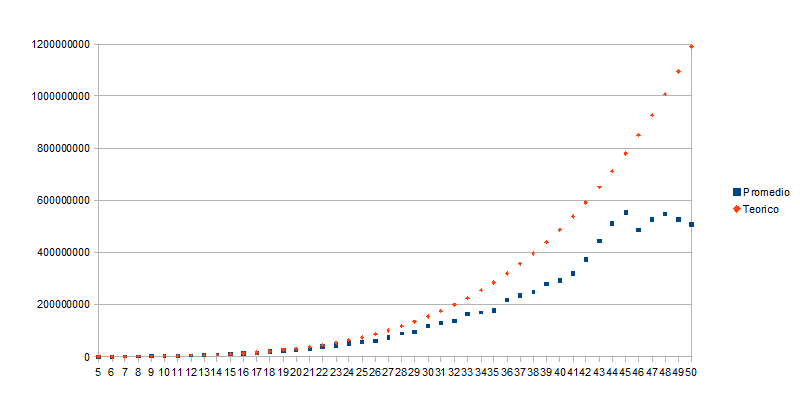
\includegraphics[scale=0.8]{grasp-tiempos-Azar.png}
\caption{Costos}
\end{figure}

\subsubsection{Grafos densos}

\begin{figure}[H]
	\centering
	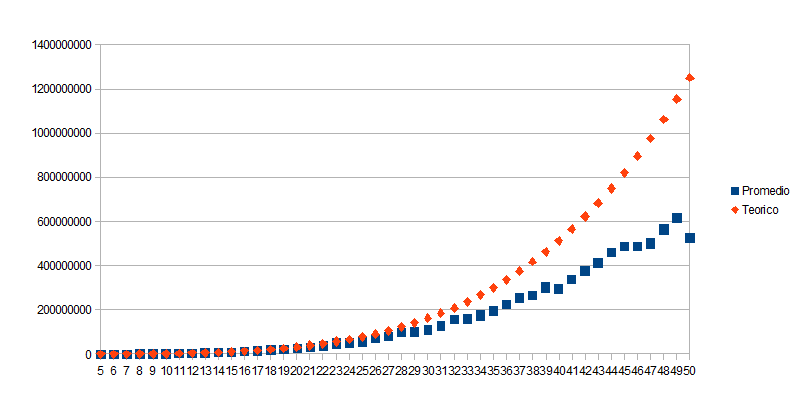
\includegraphics[scale=0.8]{grasp-tiempos-G-y-H-densos.png}
\caption{Costos}
\end{figure}

\subsubsection{G y H complementos}

\begin{figure}[H]
	\centering
	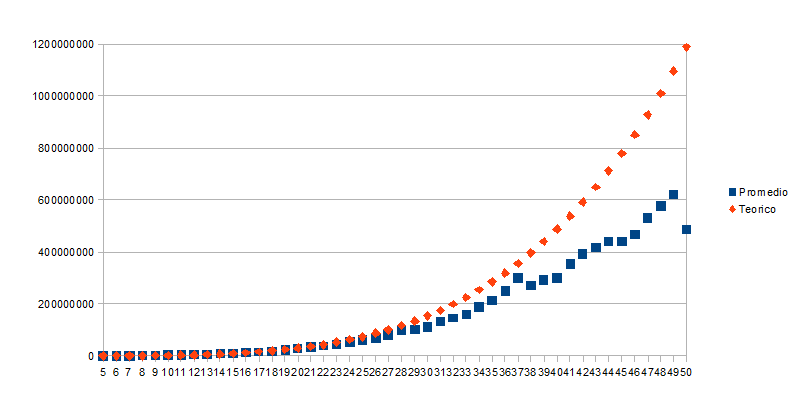
\includegraphics[scale=0.8]{grasp-tiempos-H-complemento.png}
\caption{Costos}
\end{figure}
